\chapter{Fine-Tuning Methodology}

\vspace*{1cm}

This chapter describes the methodology used to fine-tune the selected Small
Language Model. The objective of this step is to adapt
\texttt{google/flan-t5-small} to the prepared instruction-tuning dataset and to
create a training pipeline that allows the comparison of several optimization
algorithms under the same experimental conditions.

\section{Fine-Tuning Objective}

The purpose of fine-tuning is to update the parameters of a pre-trained model so
that it becomes better adapted to a specific task. In this project, the task is
instruction following. The model receives a prompt containing an instruction and,
when available, an input context. It must then generate the expected answer.

\vspace*{0.5cm}

The fine-tuning process uses the processed dataset created in the previous
chapter. The column \texttt{source\_text} is used as the model input, while the
column \texttt{target\_text} is used as the expected output. This format is
compatible with the text-to-text architecture of the T5 model family.

\section{Model and Tokenizer Loading}

The model used in this project is \texttt{google/flan-t5-small}. It is loaded
from Hugging Face using the Transformers library. The corresponding tokenizer is
also loaded in order to convert text examples into token IDs that can be processed
by the neural network.

\vspace*{0.5cm}

The tokenizer is responsible for encoding the source prompts and the target
answers. During training, the source sequence is passed to the encoder and the
target sequence is used to compute the training loss. Padding and truncation are
applied to obtain fixed-size batches suitable for GPU computation.

\section{Training Pipeline}

The training process is implemented mainly in \texttt{src/train.py}. This script
coordinates the complete fine-tuning workflow, from loading the dataset to saving
the final model and metrics. Several helper files are used to keep the
implementation organized.

\begin{figure}[H]
    \centering
    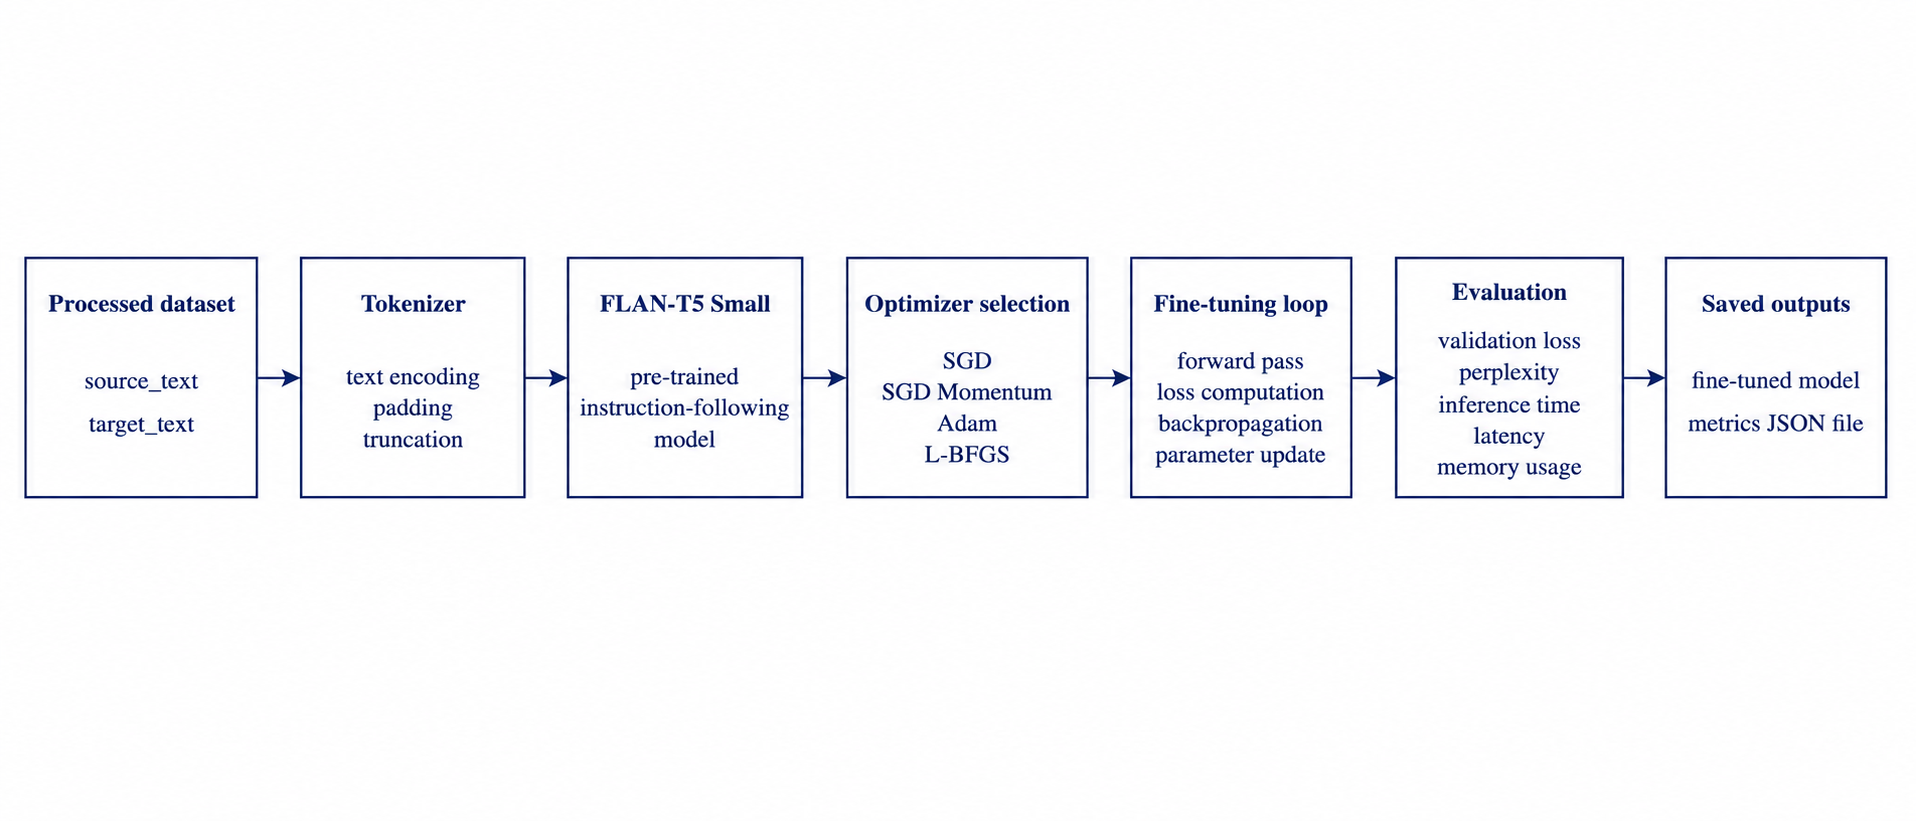
\includegraphics[width=\textwidth]{chapters/images/finetunning_flow.png}
    \caption{Fine-tuning workflow used in the project.}
    \label{fig:finetuning_workflow}
\end{figure}


\vspace*{0.5cm}

The main components of the training pipeline are:

\begin{itemize}
    \item \texttt{train.py}: controls the training execution.
    \item \texttt{training\_config.py}: defines training parameters.
    \item \texttt{model\_utils.py}: loads and saves the model.
    \item \texttt{tokenizer\_utils.py}: prepares the tokenizer and tokenized data.
    \item \texttt{optimizers.py}: selects the optimizer to use.
    \item \texttt{train\_utils.py}: contains helper functions for training.
    \item \texttt{metrics.py}: computes performance and efficiency metrics.
\end{itemize}

\section{Optimizer Selection}

One of the main goals of the project is to compare different optimization
algorithms. For this reason, the training script accepts an optimizer argument.
This makes it possible to run the same fine-tuning pipeline with different
optimization methods while keeping the dataset and model unchanged.

\vspace*{0.5cm}

The supported training commands are:

% \begin{lstlisting}[style=jsonStyle]
% python src/train.py --optimizer sgd
% python src/train.py --optimizer sgd_momentum
% python src/train.py --optimizer adam
% python src/train.py --optimizer lbfgs
% \end{lstlisting}

\begin{figure}[H]
    \centering
    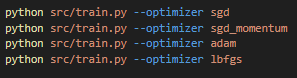
\includegraphics[width=0.55\textwidth]{chapters/images/optimizer_training_commands.png}
    \caption{Commands used to launch fine-tuning with each optimizer.}
    \label{fig:optimizer_training_commands}
\end{figure}

The script also supports running all implemented optimizers sequentially:

\begin{lstlisting}[style=jsonStyle]
python src/train.py --optimizer all
\end{lstlisting}

\section{GPU Requirement}

The fine-tuning process is designed to run on a CUDA-enabled GPU. This choice is important because transformer models require significant computation during training. For this project, an RTX 5060 was used to run the experiments. Running the experiment on CPU would be possible only for debugging, but it would be too slow for a complete optimizer comparison.

\vspace*{0.5cm}

By default, the training script stops if no GPU is available. For debugging only,
CPU execution can be enabled using:

\begin{lstlisting}[style=jsonStyle]
python src/train.py --optimizer adam --allow_cpu
\end{lstlisting}

\section{Saved Outputs}

For each optimizer, the training script saves a separate fine-tuned model. This
organization makes it possible to compare the results independently and avoids
overwriting previous experiments.

\vspace*{0.5cm}

The expected model directories are:

\begin{itemize}
    \item \texttt{results/models/flan\_t5\_sgd/}
    \item \texttt{results/models/flan\_t5\_sgd\_momentum/}
    \item \texttt{results/models/flan\_t5\_adam/}
    \item \texttt{results/models/flan\_t5\_lbfgs/}
\end{itemize}

\vspace*{0.5cm}

\clearpage

The metrics are saved separately in the \texttt{results/metrics/} directory. For
each optimizer, the expected metrics file follows this format:

\begin{lstlisting}[style=jsonStyle]
results/metrics/train_<optimizer>.json
\end{lstlisting}

\section{Methodology Summary}

The fine-tuning methodology follows a controlled experimental setup. The same
model, dataset, and evaluation process are used for all optimizers. Only the
optimization algorithm changes between experiments. This makes the comparison
more reliable because differences in the results can be linked mainly to the
chosen optimizer.

\vspace*{0.5cm}

This methodology prepares the next stage of the report, where the optimization
algorithms are explained in more detail before comparing their experimental
performance.
